\documentclass[11pt,aspectratio=169]{beamer}

% ── Theme: clean blue, minimal ────────────────────────────────────────────
\usetheme{Boadilla}
\usecolortheme{dolphin}
\definecolor{myBlue}{RGB}{0,90,160}
\setbeamercolor{structure}{fg=myBlue}
\setbeamercolor{section in toc}{fg=myBlue}
% Minimal footline: only page number on the right
\setbeamertemplate{footline}
{%
  \leavevmode%
  \hbox{%
  \begin{beamercolorbox}[wd=\paperwidth,ht=2.25ex,dp=1ex,right]{footlinecolor}%
    \insertframenumber{} / \inserttotalframenumber\hspace*{2ex}
  \end{beamercolorbox}}%
  \vskip0pt%
}
\setbeamercolor{footlinecolor}{fg=myBlue!80,bg=myBlue!10}

% ── Fonts & Packages ──────────────────────────────────────────────────────
% NOTE: Beamer auto-loads xcolor, hyperref, amsmath, geometry.
%       Do NOT load enumitem --- it breaks Beamer's list handling.
\usepackage[T1]{fontenc}
\usepackage{CJKutf8}
\usepackage{newtxtext,newtxmath}
\usepackage{microtype}
\usepackage{graphicx}
\graphicspath{{docs/}}
\usepackage{booktabs}
\usepackage{listingsutf8}
\usepackage{tikz}

% ── Code style ────────────────────────────────────────────────────────────
\definecolor{codebg}{rgb}{0.95,0.95,0.95}
\lstset{
  backgroundcolor=\color{codebg},
  basicstyle=\tiny\ttfamily,
  breaklines=true,
  extendedchars=true,
  inputencoding=utf8/latin1,
  frame=single,
  framerule=0.5pt,
  numbers=left,
  numbersep=4pt,
  numberstyle=\tiny\color{gray},
  tabsize=4,
}

% ── Fix Beamer's enumerate counter not resetting between frames ───────────
% Beamer enumerate counter is global; we reset it per-frame where needed.
\newenvironment{benumerate}
  {\setcounter{enumi}{0}\begin{enumerate}}
  {\end{enumerate}}

% ── Title info ────────────────────────────────────────────────────────────
\title[AGCommentSpy]{LLM-Based Analysis of User Comments for\\HarmonyOS Applications}
\subtitle{\textsc{AGCommentSpy} --- From Raw Reviews to Actionable Insights}
\author{Lin Wenqi \quad Hu Haozhan \quad Wang Zhaohe}
\institute{CS326 Project}
\date{\today}

\begin{document}
\begin{CJK*}{UTF8}{gbsn}

% ══════════════════════════════════════════════════════════════════════════
\begin{frame}
  \titlepage
\end{frame}

% ══════════════════════════════════════════════════════════════════════════
\begin{frame}{Outline}
  \tableofcontents
\end{frame}

% ══════════════════════════════════════════════════════════════════════════
\section{Introduction}

\begin{frame}{Motivation}
  \begin{block}{HarmonyOS Ecosystem}
    \begin{itemize}
      \item Huawei's distributed OS --- smartphones, tablets, wearables, IoT
      \item AppGallery hosts \textbf{500,000+} native HarmonyOS apps
      \item User comments are a critical feedback channel for developers
    \end{itemize}
  \end{block}

  \begin{block}{Unique Challenges of HarmonyOS}
    \begin{itemize}
      \item \textbf{Closed ecosystem:} HDC protocol, limited tooling (no \texttt{adb})
      \item \textbf{Heterogeneous devices:} phones, foldables, watches, in-vehicle
      \item \textbf{Rapid API evolution:} compatibility issues surface in reviews
    \end{itemize}
  \end{block}

  \begin{center}
    \small Existing tools target Google Play / App Store --- HarmonyOS needs its own pipeline.
  \end{center}
\end{frame}

\begin{frame}{Our Approach at a Glance}
  \begin{center}
    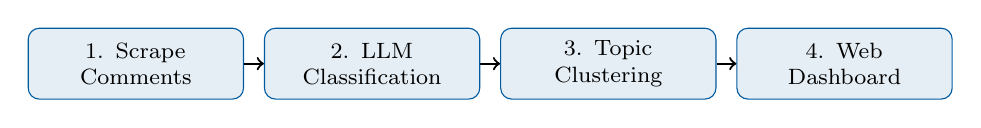
\begin{tikzpicture}[node distance=1.6cm, auto,
      block/.style={rectangle, draw=myBlue, fill=myBlue!10,
                    text width=2.5cm, text centered, rounded corners,
                    minimum height=0.9cm, font=\footnotesize}]
      \node[block] (scrape) {1. Scrape\\Comments};
      \node[block, right of=scrape, xshift=1.4cm] (classify) {2. LLM\\Classification};
      \node[block, right of=classify, xshift=1.4cm] (cluster) {3. Topic\\Clustering};
      \node[block, right of=cluster, xshift=1.4cm] (dash) {4. Web\\Dashboard};
      \draw[->, thick] (scrape) -- (classify);
      \draw[->, thick] (classify) -- (cluster);
      \draw[->, thick] (cluster) -- (dash);
    \end{tikzpicture}
  \end{center}

  \begin{block}{Key Insight}
    Use UI automation to collect reviews + LLM to classify \& cluster
    $\rightarrow$ transform \textbf{unstructured reviews} into \textbf{actionable developer insights}.
  \end{block}
\end{frame}

% ══════════════════════════════════════════════════════════════════════════
\section{Contributions}

\begin{frame}{Contributions}
  \begin{benumerate}
    \item \textbf{UI-automation crawler} --- reliably scrapes AppGallery comments via \texttt{hmdriver2} + HDC
    \item \textbf{LLM classification pipeline} --- multi-dimensional sentiment analysis + actionable suggestions
    \item \textbf{Two-stage clustering} --- intra-bucket grouping + cross-batch refinement
    \item \textbf{Interactive web dashboard} --- aggregated results in intuitive visual format
    \item \textbf{Curated dataset} --- \textbf{10,000+} comments across 8 categories on HarmonyOS
  \end{benumerate}
\end{frame}

% ══════════════════════════════════════════════════════════════════════════
\section{System Architecture}

\begin{frame}{System Architecture --- Overview}
  \begin{figure}
    \centering
    \fbox{\begin{minipage}{0.92\textwidth}\centering\small
      \textbf{Comment Scraping}
      $\rightarrow$
      \textbf{LLM Classification}
      $\rightarrow$
      \textbf{Topic Clustering}
      $\rightarrow$
      \textbf{Web Dashboard}
      \\[3pt]
      \scriptsize
      HDC + hmdriver2 \quad|\quad
      LLM API (JSON mode) \quad|\quad
      2-stage LLM cluster \quad|\quad
      Python HTTP + Vanilla JS
    \end{minipage}}
  \end{figure}

  \begin{columns}[T]
    \begin{column}{0.5\textwidth}
      \textbf{Technology Stack}
      \begin{itemize}
        \item \texttt{hmdriver2} + HDC --- device automation
        \item \texttt{lxml} + XPath --- UI parsing
        \item OpenAI-compatible API --- LLM calls
        \item Python 3.13 --- all backend logic
        \item Vanilla JS + SVG --- frontend
      \end{itemize}
    \end{column}
    \begin{column}{0.5\textwidth}
      \textbf{Data Flow}
      \begin{itemize}
        \item Raw comments $\rightarrow$ JSON files
        \item Batch LLM classification (10/batch)
        \item Classification $\rightarrow$ clustering
        \item REST API $\rightarrow$ dashboard
      \end{itemize}
    \end{column}
  \end{columns}
\end{frame}

% ──────────────────────────────────────────────────────────────────────────
\subsection{Comment Scraping}

\begin{frame}[fragile]{Stage 1: Comment Scraping}
  \begin{columns}[T]
    \begin{column}{0.48\textwidth}
      \textbf{How it works}
      \begin{itemize}
        \item Launch AppGallery via deep-link URL
        \item \textbf{Configurable swipes} to load reviews (max~500)
        \item Parse UI hierarchy (JSON $\rightarrow$ XML, XPath)
        \item Extract: username, rating, text, date, device
        \item \textbf{Auto-expand} truncated long comments
        \item Save per-app JSON files
      \end{itemize}
    \end{column}
    \begin{column}{0.52\textwidth}
      \textbf{Scraping Loop (simplified)}
      \begin{lstlisting}[language=Python]
def scrape_comments(driver, max_swipes=50):
    all_comments = []
    for i in range(max_swipes):
        driver.swipe(...)
        layout = driver.dump_hierarchy()
        xml = json2xml(layout)
        for node in xml.xpath(COMMENT_XPATH):
            c = parse_comment(node)
            all_comments.append(c)
    return all_comments
      \end{lstlisting}
    \end{column}
  \end{columns}
\end{frame}

% ──────────────────────────────────────────────────────────────────────────
\subsection{LLM Classification}

\begin{frame}{Stage 2: LLM-Based Classification}
  \scriptsize
  \begin{columns}[T]
    \begin{column}{0.45\textwidth}
      \textbf{Goal}\\
      Raw app reviews $\rightarrow$ structured developer insights

      \vspace{0.12cm}
      \textbf{Classification}
      \begin{itemize}
        \setlength\itemsep{0pt}
        \item \textbf{Sentiment:} \textcolor{green!60!black}{Positive},
              \textcolor{red!60!black}{Negative}, \textcolor{gray}{Neutral}
        \item \textbf{7 dimensions:}
      \end{itemize}
      \vspace{-0.22cm}
      \begin{columns}[T,onlytextwidth]
        \begin{column}{0.5\textwidth}
          \begin{itemize}\tiny
            \setlength\itemsep{0pt}
            \item Functional Experience
            \item System Compatibility
            \item Stability \& Performance
            \item UI \& Interaction
          \end{itemize}
        \end{column}
        \begin{column}{0.5\textwidth}
          \begin{itemize}\tiny
            \setlength\itemsep{0pt}
            \item Operations \& Policies
            \item Appreciation
            \item Content Ecosystem
          \end{itemize}
        \end{column}
      \end{columns}

      \vspace{0.08cm}
      \textbf{Structured Output}
      \begin{itemize}
        \setlength\itemsep{0pt}
        \item Pain point + actionable suggestion
        \item Comment ID for traceability
      \end{itemize}

      \vspace{0.08cm}
      \textbf{Reliability}
      \begin{itemize}
        \setlength\itemsep{0pt}
        \item JSON schema, 10 comments/batch
        \item Auto-repair malformed responses
      \end{itemize}
    \end{column}
    \begin{column}{0.55\textwidth}
      \begin{exampleblock}{Example}
        \scriptsize
        \textbf{Raw review}\\
        ``The HarmonyOS version crashes when opening videos, and landscape mode is poorly adapted.''

        \vspace{0.1cm}
        \textbf{LLM classification output}
        \begin{itemize}
          \setlength\itemsep{1pt}
          \item \textbf{Sentiment:} \textcolor{red!60!black}{Negative}
          \item \textbf{Dimension:} Stability \& Performance
          \item \textbf{Pain point:} Video playback crashes
          \item \textbf{Suggestion:} Check crash logs; improve landscape adaptation
        \end{itemize}
      \end{exampleblock}
    \end{column}
  \end{columns}
\end{frame}

% ──────────────────────────────────────────────────────────────────────────
\subsection{Topic Clustering}

\begin{frame}{Stage 3: Two-Stage Topic Clustering}
  \footnotesize
  \begin{columns}[T]
    \begin{column}{0.38\textwidth}
      \textbf{Initial attempt: word-embedding clustering}
      \begin{itemize}
        \setlength\itemsep{0pt}
        \item Sentence-BERT + KMeans/DBSCAN
        \item \textbf{Failed:} same root cause, different wording $\rightarrow$ far apart in vector space $\rightarrow$ split into different clusters
      \end{itemize}

      \vspace{0.1cm}
      \textbf{Our approach: LLM-as-clusterer}
      \begin{itemize}
        \setlength\itemsep{2pt}
        \item \textbf{Stage 1:} partition by (dimension, sentiment); LLM clusters items within each bucket in batches of 18
        \item \textbf{Stage 2:} merges overlapping clusters across batches and standardizes topic names      
        \end{itemize}
    \end{column}
    \begin{column}{0.55\textwidth}
      \begin{exampleblock}{Example}
        \scriptsize
        \textbf{cluster\_name:} 好友信息功能缺失\\
        \textbf{canonical\_issue:} 鸿蒙版微信缺少好友来源、共同群聊、添加好友时间等常用功能\\
        \textbf{size:} 2

        \vspace{0.1cm}
        \begin{tabular}{@{}p{0.48\textwidth}p{0.48\textwidth}@{}}
          \scriptsize \textbf{\#264} \quad \textit{华为畅享 90 Pro Max} &
          \scriptsize \textbf{\#272} \quad \textit{HUAWEI Pura 70 Pro+} \\[2pt]
          \scriptsize ``好友来源、好友共同群聊、添加好友时间等都没有，求更新'' &
          \scriptsize ``连朋友资料都没，版本比别人低...'' \\
        \end{tabular}
      \end{exampleblock}
    \end{column}
  \end{columns}
\end{frame}

% ──────────────────────────────────────────────────────────────────────────
\subsection{Web Dashboard}

\begin{frame}{Stage 4: Web Dashboard}
  \begin{columns}[T]
    \begin{column}{0.45\textwidth}
      \textbf{Four Tabs}
      \begin{benumerate}
        \item \textbf{Overview}
              \begin{itemize}\footnotesize
                \item Total comments, classified count
                \item Donut chart (sentiment)
                \item Bar chart (dimensions)
              \end{itemize}
        \item \textbf{Comments}
              \begin{itemize}\footnotesize
                \item Paginated list + full-text search
                \item Username, rating, date, device
              \end{itemize}
      \end{benumerate}
    \end{column}
    \begin{column}{0.55\textwidth}
      \setcounter{enumi}{2}
      \begin{enumerate}
        \item \textbf{Analysis}
              \begin{itemize}\footnotesize
                \item Dimension-filtered pain points
                \item LLM-generated \textbf{actionable suggestions}
              \end{itemize}
        \item \textbf{Clusters}
              \begin{itemize}\footnotesize
                \item Topics by dimension $\times$ sentiment
                \item Expandable sample members
              \end{itemize}
      \end{enumerate}

      \vspace{0.3cm}
      \begin{block}{Tech Stack}
        \footnotesize
        Vanilla JS (no framework) + inline SVG charts\\
        Python HTTP server + REST API endpoints
      \end{block}
    \end{column}
  \end{columns}
\end{frame}

% ══════════════════════════════════════════════════════════════════════════
\section{Results}

\begin{frame}{Results --- Dashboard Overview}
  \begin{columns}[T]
    \begin{column}{0.55\textwidth}
      \begin{figure}
        \centering
        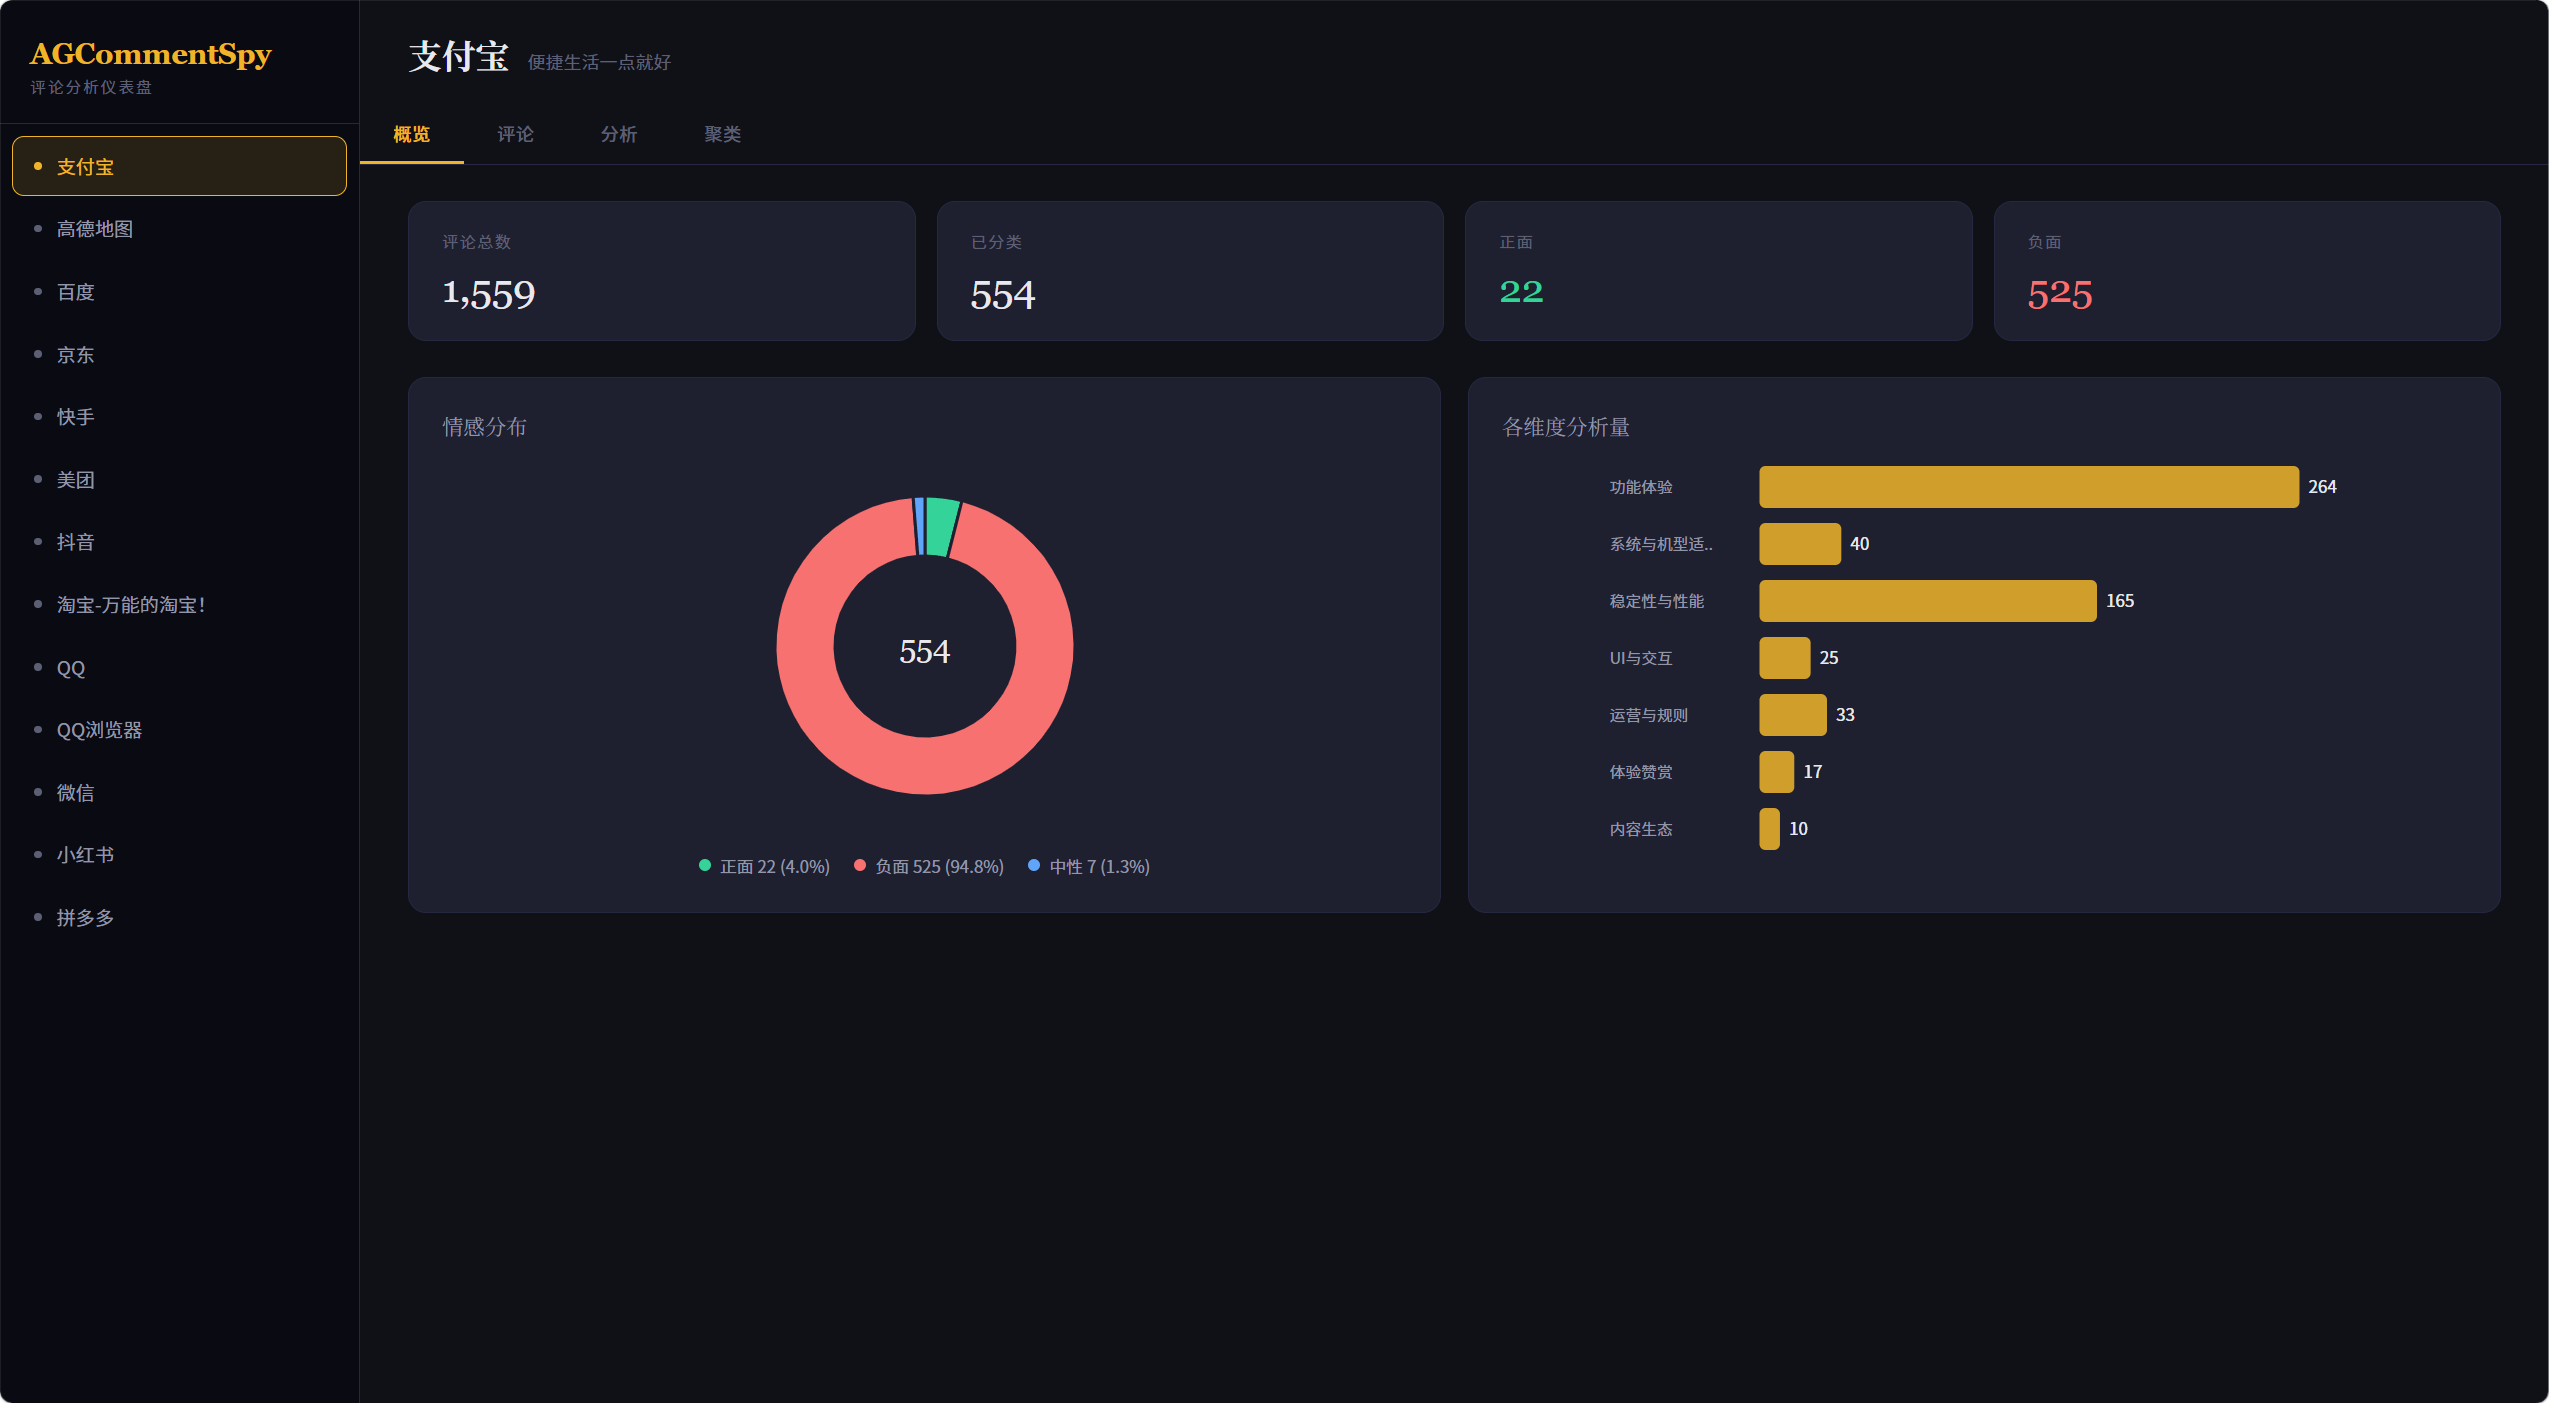
\includegraphics[width=\textwidth]{overview.png}
        \caption{Overview --- aggregate statistics and charts}
      \end{figure}
    \end{column}
    \begin{column}{0.45\textwidth}
      \begin{itemize}
        \item \textbf{Dataset:} \textbf{10,000+} comments across \textbf{45+} apps in 8 categories
        \item \textbf{Sentiment distribution} visualized as an SVG donut chart
        \item \textbf{Dimension breakdown} shown as a horizontal bar chart
        \item One-click access to total/classified counts
      \end{itemize}
    \end{column}
  \end{columns}
\end{frame}

\begin{frame}{Results --- Analysis \& Clusters}
  \begin{columns}[T]
    \begin{column}{0.5\textwidth}
      \begin{figure}
        \centering
        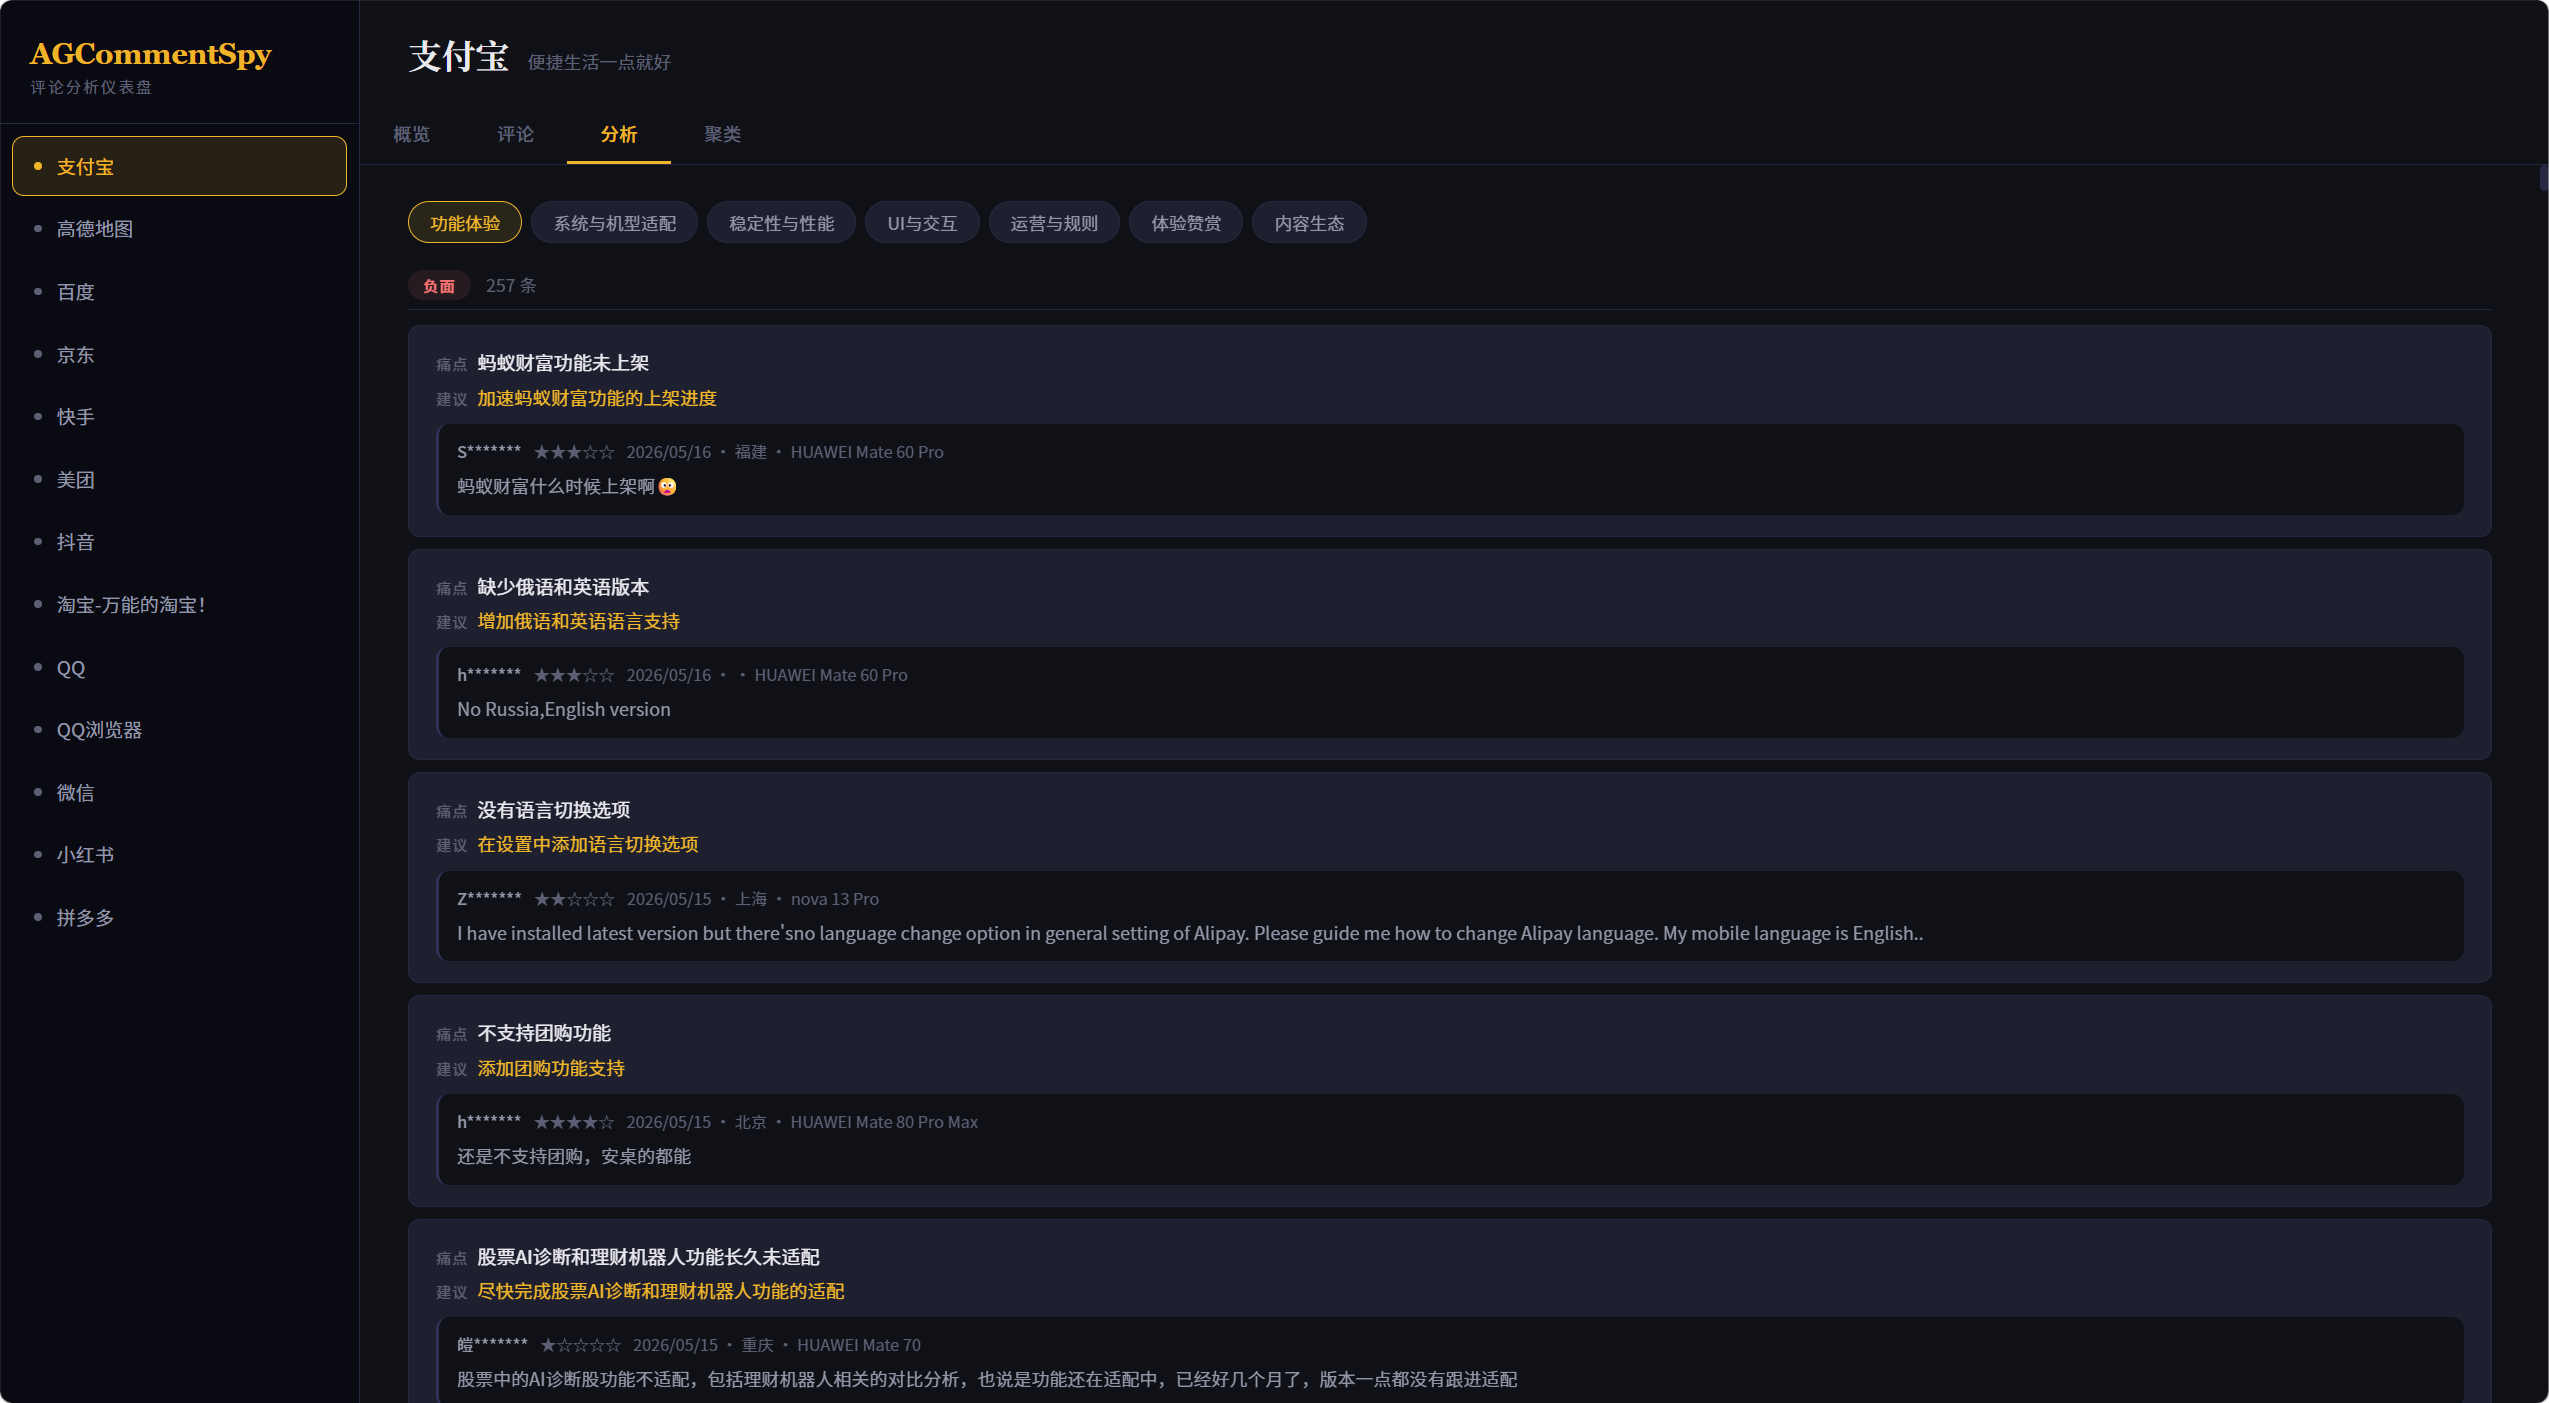
\includegraphics[width=\textwidth]{analysis.png}
        \caption{Analysis --- per-dimension issues with suggestions}
      \end{figure}
    \end{column}
    \begin{column}{0.5\textwidth}
      \begin{figure}
        \centering
        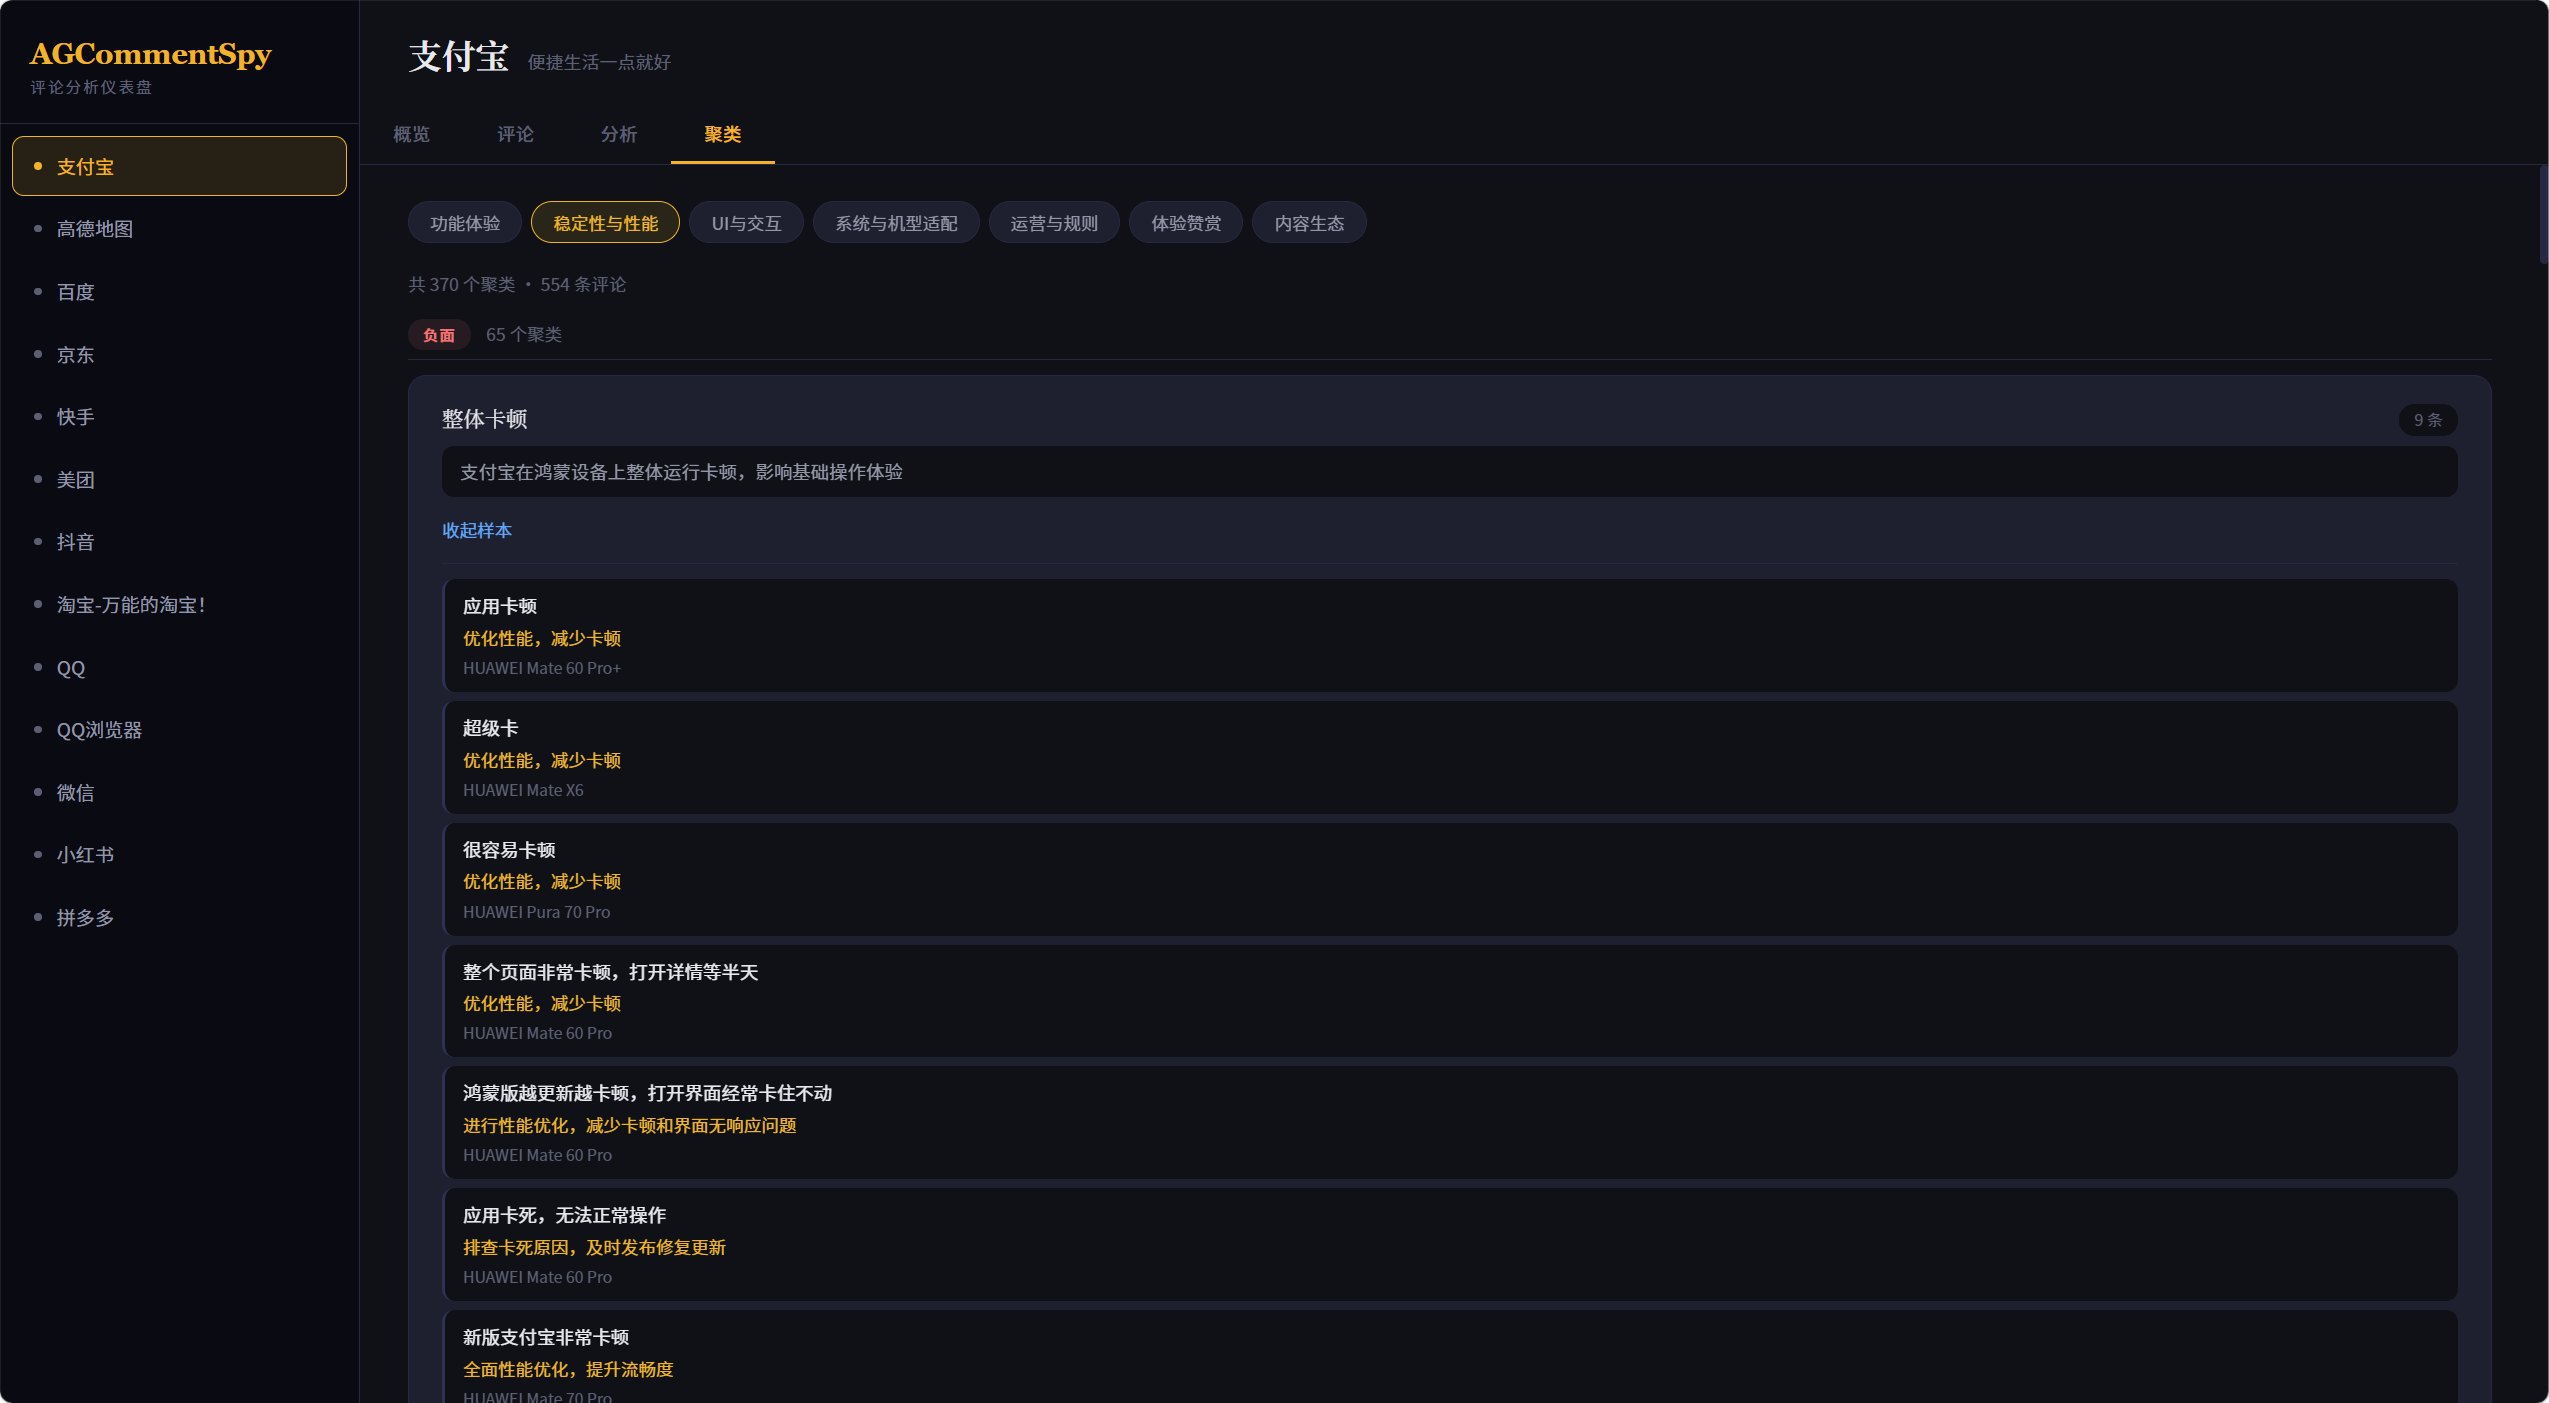
\includegraphics[width=\textwidth]{cluster.png}
        \caption{Clusters --- grouped issues with canonical descriptions}
      \end{figure}
    \end{column}
  \end{columns}
\end{frame}

% ══════════════════════════════════════════════════════════════════════════
\section{Evaluation \& Discussion}

\begin{frame}{Evaluation \& Discussion}
  \begin{block}{Classification}
    \begin{itemize}
      \item 7 dimensions balance \textbf{granularity} with \textbf{actionability}
      \item Every negative issue $\rightarrow$ concrete \texttt{Actionable\_Suggestion}
    \end{itemize}
  \end{block}

  \begin{block}{Clustering}
    \begin{itemize}
      \item Word-embedding clustering separated same-root-cause items (lexical, not semantic)
      \item LLM-as-clusterer reasons about root causes, merging despite vocabulary variance
      \item Two-stage design: focused sub-problems + lightweight reconciliation
    \end{itemize}
  \end{block}
\end{frame}

% ══════════════════════════════════════════════════════════════════════════
\section{Conclusion \& Future Work}

\begin{frame}{Conclusion}
  \begin{block}{What We Built}
    \textsc{AGCommentSpy} --- end-to-end pipeline that transforms
    \textbf{unstructured AppGallery reviews} into \textbf{actionable developer
    insights} via UI automation + LLM-based NLP.
  \end{block}

  \begin{block}{Key Takeaways}
    \begin{itemize}
      \item UI automation compensates for the \textbf{lack of public APIs} on HarmonyOS
      \item LLMs enable \textbf{zero-shot} fine-grained classification of user reviews
      \item Two-stage clustering turns \textbf{scattered comments} into \textbf{coherent topics}
      \item Lightweight web dashboard makes results \textbf{accessible to developers}
    \end{itemize}
  \end{block}
\end{frame}

\begin{frame}{Future Work}
  \begin{benumerate}
    \item \textbf{Automated labeling} --- human-annotated gold standard for evaluation
    \item \textbf{LLM comparison} --- benchmark multiple providers on cost-quality
    \item \textbf{Incremental scraping} --- only scrape new comments since last run
    \item \textbf{Developer workflow integration} --- auto-file findings to GitHub Issues / Jira
  \end{benumerate}
\end{frame}

% ══════════════════════════════════════════════════════════════════════════
\begin{frame}[plain]
  \begin{center}
    \Huge\color{myBlue} Thank You!

    \vspace{1cm}
    \normalsize\color{black}
    Questions \& Discussion

    \vspace{1.5cm}
    \small
    \textsc{AGCommentSpy} --- CS326 Project
  \end{center}
\end{frame}

\end{CJK*}
\end{document}